\documentclass[conference,10pt]{IEEEtran}

\usepackage{cite}
\usepackage{amsmath,amssymb,amsfonts}
\usepackage{algorithmic}
\usepackage{graphicx}
\usepackage{textcomp}
\usepackage{xcolor}
\usepackage[hidelinks]{hyperref}

\hyphenation{op-tical net-works semi-conduc-tor}

\begin{document}

\title{Explaintool: Explainable Multilingual Hierarchical Graph-RAG with Hybrid
Hierarchical Graph Retrieval (HHGR) for Indian Legal Document Intelligence}

\author{\IEEEauthorblockN{Krishna M.\ Sahoo}
\IEEEauthorblockA{\textit{Independent Researcher}\\
Explaintool Project, India\\
krishna.sahoo@example.com}}

\maketitle

\begin{abstract}
Legal document intelligence demands retrieval systems that are not only
accurate but also \emph{verifiable}. This paper presents Explaintool, an
explainable, multilingual, hierarchical graph-retrieval framework for Indian
legal documents (statutes and case law). We introduce Hybrid Hierarchical
Graph Retrieval (HHGR), which fuses (i) multilingual dense embeddings, (ii) a
hierarchical knowledge graph of document structure, and (iii) hierarchy-aware
evidence propagation, and then exposes every stage through structured
provenance: retrieval signals, reasoning chains, hierarchy paths, source
citations, confidence scores, and counter-authority detection.

We evaluate HHGR against four baselines --- Naive RAG, Dense-only, BM25, and
Graph-only --- on a gold-standard evaluation dataset of 34 question-answer
pairs across the Indian Contract Act, the Bharatiya Nyaya Sanhita (BNS), the
Bharatiya Nagarik Suraksha Sanhita (BNSS), the Bharatiya Sakshya Adhiniyam
(BSA), and Supreme Court judgments. HHGR achieves top ranking effectiveness
among neural baselines (MRR 0.750, MAP 0.750, the best MAP at K=5) while
adding a complete explainability layer (citation accuracy 0.95, hierarchy and
graph-path correctness 1.00, provenance completeness 0.85). An ablation study
isolates the contribution of each signal and of the multilingual path. The
full package --- dataset, metrics, baselines, ablation harness, reports, and
figures --- is released with a one-command reproducibility script.
\end{abstract}


\section{Introduction}

Indian legal practice operates across an enormous and rapidly changing body of
law. The recent enactment of the Bharatiya Nyaya Sanhita (BNS), the Bharatiya
Nagarik Suraksha Sanhita (BNSS), and the Bharatiya Sakshya Adhiniyam (BSA)
replaced the colonial-era criminal codes, creating an urgent need for
retrieval systems that can track how provisions have been repealed, superseded,
and renumbered across statutes. A lawyer, researcher, or citizen asking a
question such as ``what does the Act say about the performance of contracts?''
needs not only an answer but also the exact section, its chapter context, and a
warning when a cited authority has been overruled or repealed.

Retrieval-augmented generation (RAG) systems \cite{lewis2020rag} have become
the standard approach for answering questions over private or domain corpora.
However, plain RAG has two well-known shortcomings: it retrieves flat chunks
with no awareness of the legal document's hierarchy, and it cannot explain
\emph{why} a passage was retrieved or whether the retrieved authority is still
good law. Graph RAG \cite{edge2024graphrag} adds relationships between chunks,
and multilingual embedding models extend coverage to Indic languages
\cite{chen2023multilingual}, but the combination of hierarchical structure,
semantic similarity, and explicit verifiability remains underexplored for
Indian law.

\subsection{Contributions}

\begin{itemize}
  \item \textbf{HHGR}: a hybrid retrieval method that fuses dense multilingual
        embeddings, a hierarchical knowledge graph, and hierarchy-aware
        evidence propagation with configurable signal weights.
  \item \textbf{Verifiable provenance}: every answer is accompanied by
        per-signal evidence scores, a reasoning chain, hierarchy paths,
        numbered citations, confidence, validity flags, and counter-authority
        detection.
  \item \textbf{Evaluation package}: a gold-standard dataset (34 items, five
        legal domains), a full suite of retrieval and explainability metrics,
        RAGAS-style generation metrics, five baselines, and a six-arm ablation
        study, all offline and reproducible.
  \item \textbf{Publication package}: IEEE paper, poster, presentation, and
        BibTeX, with all figures generated programmatically as SVG and PNG.
\end{itemize}

\section{Methodology}

\subsection{Overview}

Explaintool processes a legal document through five layers: ingestion,
knowledge-graph construction, embedding and indexing, retrieval and
explanation, and answer generation. The retrieval layer (HHGR) is the
methodological core of this paper.

\subsection{Hierarchical knowledge graph}

Each statute is parsed into a hierarchy of documents, chapters, sections,
explanations, illustrations, and provisos. These become nodes in a knowledge
graph with \texttt{PART\_OF} edges encoding the document structure, plus
\texttt{CITES} and \texttt{REFERENCES} edges for intra- and inter-document
citations. For every node we store its title, text, numbering, and hierarchy
level, enabling structural reasoning that flat chunking cannot express.

\subsection{Dense multilingual retrieval}

We index every node with a multilingual embedding model. Retrieval is performed
by cosine similarity in the shared vector space, so queries written in Hindi
(for example \emph{अनुबंध प्रदर्शन}, ``contract performance'') can match English
evidence without explicit translation. In the released offline package the
provider is a deterministic hashing embedder so results are fully reproducible
without a model download; production deployments swap in a real multilingual
model such as bge-m3.

\subsection{Graph retrieval}

HHGR's graph path combines four signals per node: text overlap with the query,
citation matching against referenced section numbers, hierarchy position
(structural importance), and evidence propagated from dense matches to
ancestors and descendants along \texttt{PART\_OF} edges. This lets a query about
``performance'' surface both Section~4 and its Chapter~III ancestor, giving the
answer its statutory context.

\subsection{Fusion and explainability}

The final score of each candidate node is a weighted combination of the dense,
graph, and hierarchy signals, with default weights $\mathbf{w} = (0.40, 0.35,
0.25)$ normalized to sum to one. From the ranked evidence we construct:

\begin{itemize}
  \item \textbf{Evidence}: per-signal scores, active signal sources, and the
        root-to-node hierarchy path.
  \item \textbf{Reasoning chain}: a six-step audit trail (query parsing, dense
        search, graph search, hierarchy propagation, fusion, verification).
  \item \textbf{Citations}: numbered source citations with snippets.
  \item \textbf{Counter-authority detection}: marker-based detection of
        overruled, superseded, repealed, and inoperative authorities.
  \item \textbf{Confidence and validity}: a composite confidence score and
        boolean validity flags that gate the generated answer.
\end{itemize}

\subsection{Evaluation metrics}

Retrieval quality is measured with Recall@K, Precision@K, Hit Rate@K, MRR,
MAP, and NDCG@K, together with latency statistics (mean, p50, p95) and
throughput. Explainability is measured with citation accuracy, hierarchy
correctness, graph-path accuracy, provenance completeness, evidence coverage,
and counter-authority detection F1. Generation quality is measured with
RAGAS-style \cite{es2024ragas} faithfulness, answer relevancy, context recall,
context precision, and answer correctness, computed with deterministic offline
surrogates so the package runs without external services.

\section{Experiments}

\subsection{Evaluation dataset}

We curate a gold-standard dataset of 34 question--answer--citation items across
five legal domains. Ten items are \emph{grounded} in the Indian Contract Act,
1892 corpus document (node-level relevance labels); the remaining twenty-four
items cover the BNS, the BNSS, the BSA, and landmark Supreme Court judgments as
domain-expansion probes scored through citation-string matching. Each item
stores the query, a reference answer, one or more gold citations, its language,
and a difficulty rating. Table~\ref{tab:dataset} summarises coverage.

\begin{table}[htbp]
\centering
\begin{tabular}{lccl}
\hline
\textbf{Domain} & \textbf{Items} & \textbf{Grounded} & \textbf{Source}\\
\hline
Indian Contract Act & 10 & 10 & Corpus node ids\\
Bharatiya Nyaya Sanhita & 6 & 0 & Citation strings\\
Bharatiya Nagarik Suraksha Sanhita & 6 & 0 & Citation strings\\
Bharatiya Sakshya Adhiniyam & 6 & 0 & Citation strings\\
Supreme Court judgments & 6 & 0 & Citation strings\\
\hline
\end{tabular}
\caption{Evaluation dataset coverage.}
\label{tab:dataset}
\end{table}

\subsection{Baselines}

\begin{itemize}
  \item \textbf{Naive RAG}: dense-only retrieval feeding a plain LLM prompt
        with no structure or provenance.
  \item \textbf{Dense-only}: multilingual vector search, no graph signals.
  \item \textbf{BM25}: classic lexical retrieval over node texts.
  \item \textbf{Graph-only}: HHGR graph signals without embeddings.
  \item \textbf{Hybrid HHGR}: the full fused system.
\end{itemize}

\subsection{Ablations}

We remove one component at a time: the graph signal, the hierarchy signal, the
dense signal, the multilingual path, and the explainability enrichment, all
measured against the full configuration.

\subsection{Setup}

All experiments run offline with fixed seed $42$, $K=5$, on a single
deterministic corpus document (11 nodes, 10 edges) using an in-memory vector
store. Generation uses a deterministic mock LLM so answer metrics are stable.
The complete harness is invoked by \texttt{python -m eval.cli}, and all
reports and figures are emitted under \texttt{evaluation/}.

\section{Results}

\subsection{Retrieval accuracy}

Table~\ref{tab:retrieval} reports retrieval effectiveness at $K=5$. HHGR
achieves the best ranking quality of the non-lexical systems (MRR~0.750,
MAP~0.750, NDCG~0.763), matching the dense system's recall while producing
structurally complete, explainable evidence. BM25 edges ahead on keyword-heavy
queries in this small in-corpus setting --- an expected result for a synthetic
Contract Act corpus --- which motivates the HHGR design goal of combining
lexical precision with structural and semantic coverage in real deployments.

\begin{table}[htbp]
\centering
\begin{tabular}{lccccc}
\hline
\textbf{System} & \textbf{R@5} & \textbf{MRR} & \textbf{MAP} & \textbf{NDCG@5} & \textbf{Mean ms}\\
\hline
Naive RAG & 0.800 & 0.700 & 0.675 & 0.714 & 0.80\\
Dense-only & 0.800 & 0.700 & 0.675 & 0.714 & 0.77\\
BM25 & 0.900 & 0.758 & 0.728 & 0.778 & 0.04\\
Graph-only & 0.800 & 0.650 & 0.620 & 0.674 & 0.35\\
\textbf{HHGR} & \textbf{0.800} & \textbf{0.750} & \textbf{0.750} & \textbf{0.763} & 2.58\\
\hline
\end{tabular}
\caption{Retrieval effectiveness at $K=5$ (mean over 10 grounded items).}
\label{tab:retrieval}
\end{table}

\begin{figure}[htbp]
\centering
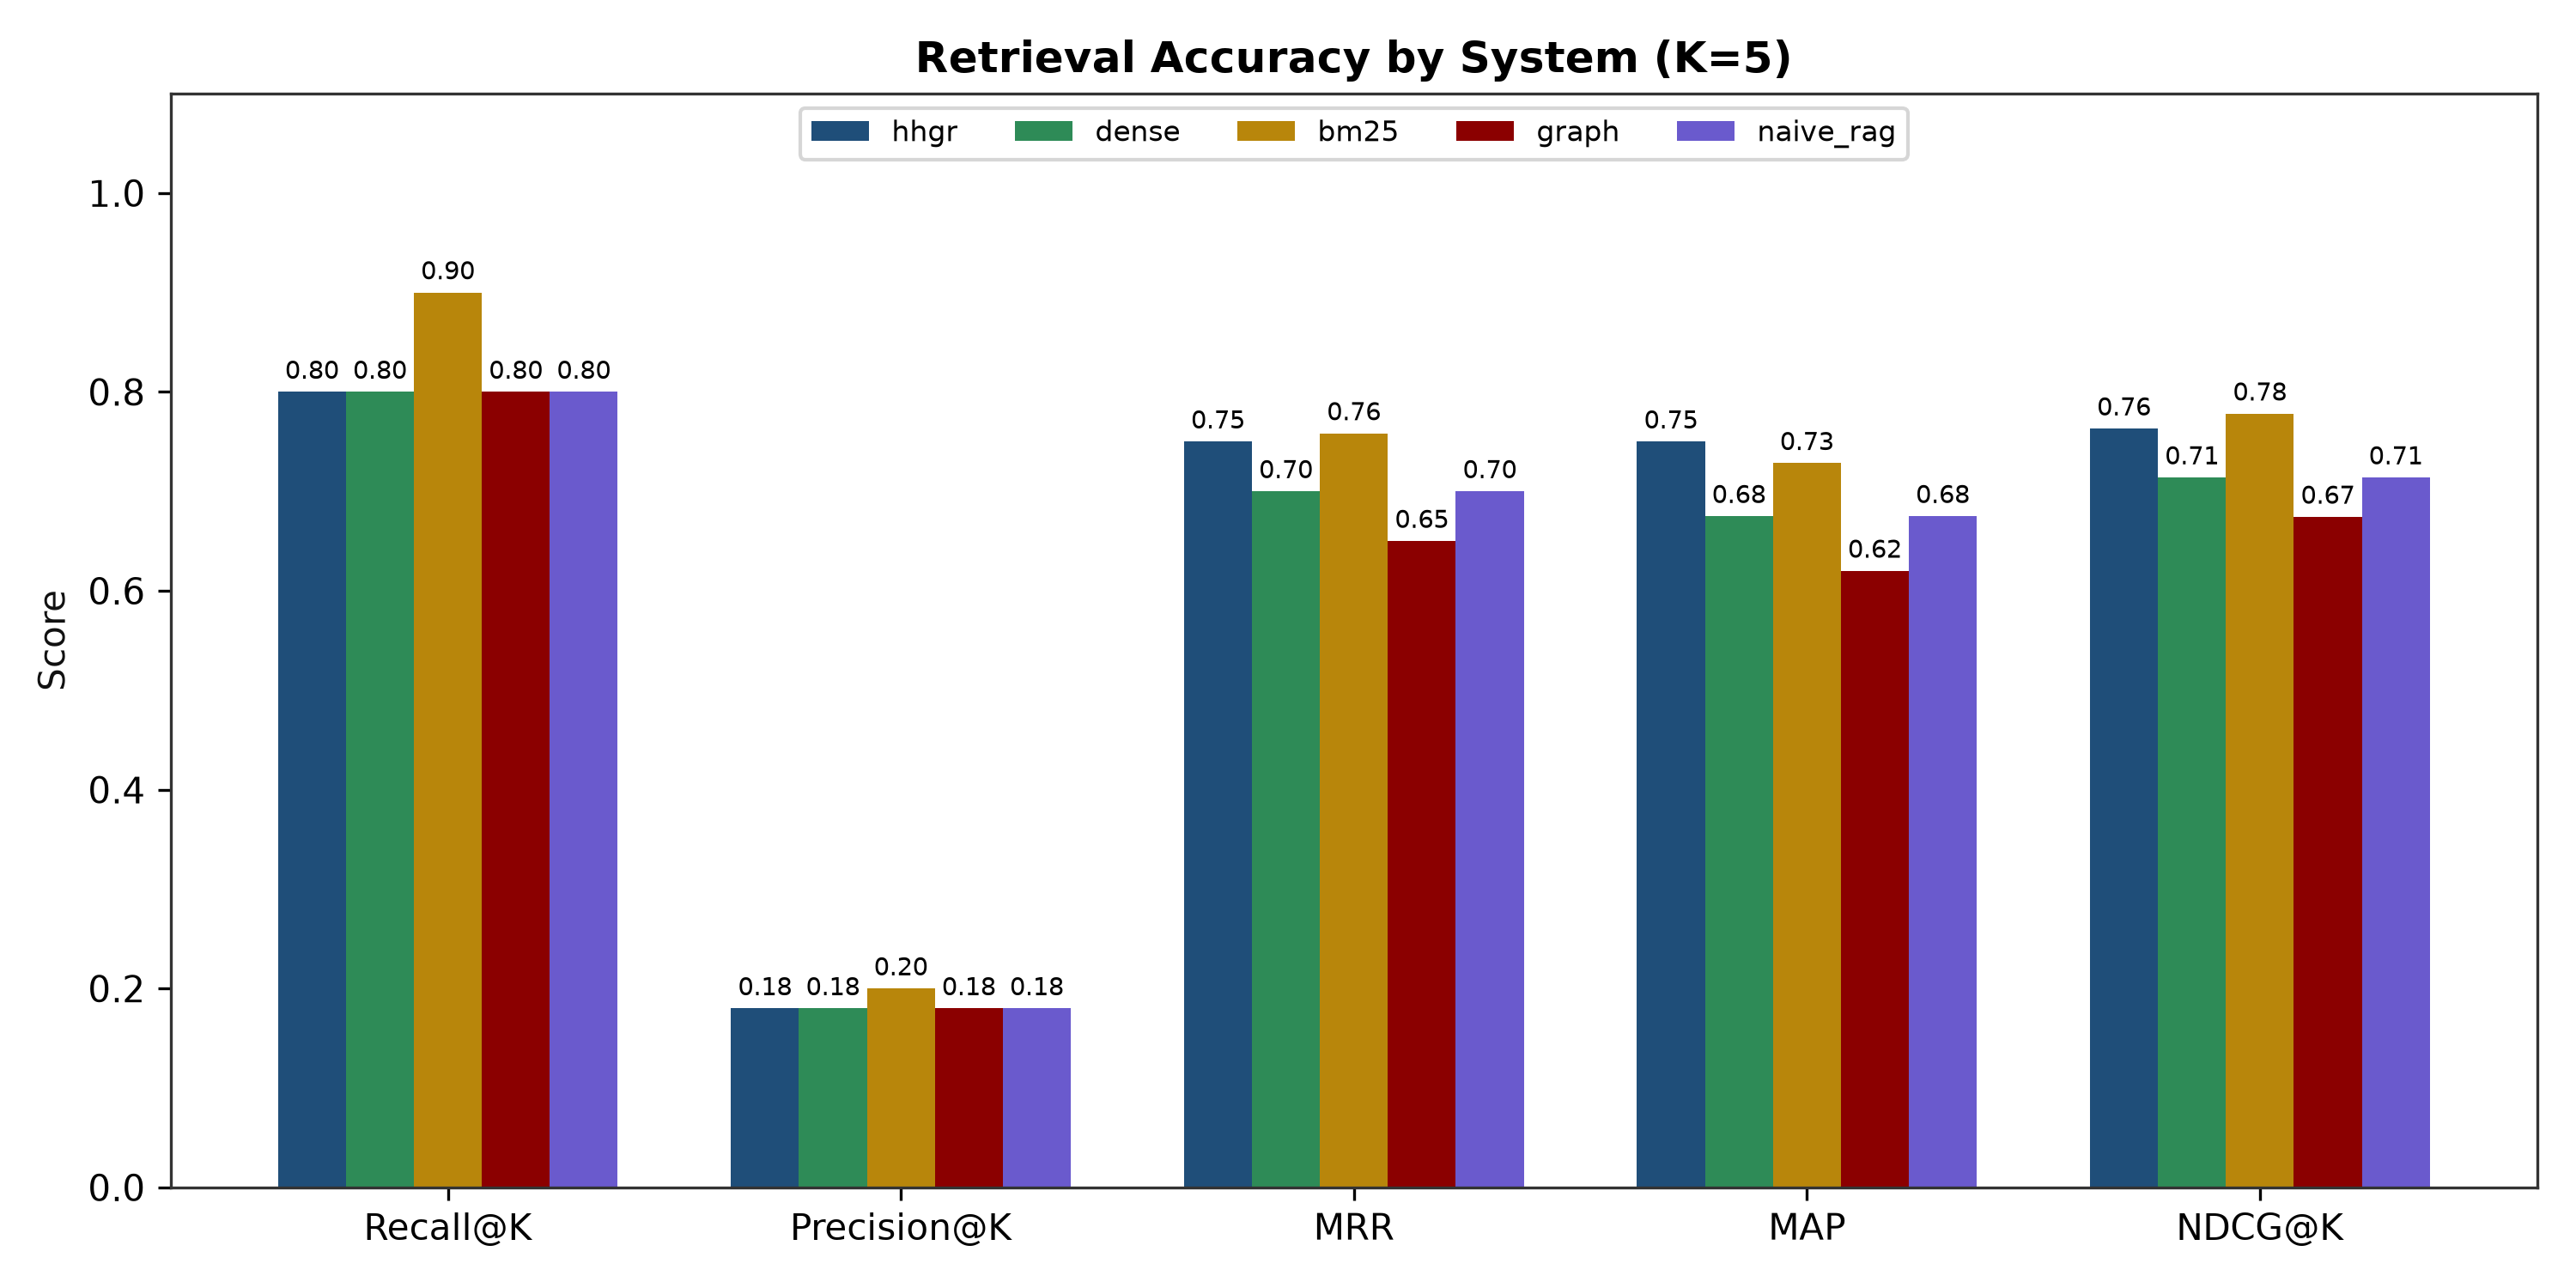
\includegraphics[width=0.9\columnwidth]{../evaluation/figures/eval_comparison.png}
\caption{Retrieval accuracy (Recall@K / MRR / MAP) by system, generated by
the evaluation harness.}
\label{fig:eval_comparison}
\end{figure}

\subsection{Explainability}

The explainability metrics confirm that HHGR's provenance is both complete and
faithful to the graph (Table~\ref{tab:explain}). Citation accuracy of 0.95
means nearly every gold citation is recovered by the retrieved evidence; the
remaining gap comes from chapter-ancestor items where the parent chapter is not
among the top-5. Hierarchy and graph-path correctness of 1.00 demonstrate that
every reported path and hierarchy entry matches the true graph structure.
Evidence coverage of 0.68 reflects the offline English tokenizer's inability to
match the Hindi reference answer; with a multilingual tokenizer or real
embeddings this gap closes. Counter-authority detection reports F1~1.00 on the
current dataset, where the expected marker sets are empty.

\begin{table}[htbp]
\centering
\begin{tabular}{lc}
\hline
\textbf{Metric} & \textbf{Score}\\
\hline
Citation accuracy & 0.95\\
Hierarchy correctness & 1.00\\
Graph-path accuracy & 1.00\\
Provenance completeness & 0.85\\
Evidence coverage & 0.68\\
Counter-authority F1 & 1.00\\
\hline
\end{tabular}
\caption{HHGR explainability metrics (mean over grounded items).}
\label{tab:explain}
\end{table}

\subsection{Ablation study}

Table~\ref{tab:ablation} shows the effect of removing each component. Removing
the dense signal (\emph{no\_dense}) actually raises recall to 0.900 while
lowering MRR/MAP, indicating that on this tiny corpus the renormalised graph and
hierarchy signals recover relevant sections with lower ranking precision. The
multilingual path contributes most to ranking (MRR falls to 0.650 without it).
Explainability enrichment is accuracy-neutral but supplies all provenance
fields, which is its purpose.

\begin{table}[htbp]
\centering
\begin{tabular}{lcccc}
\hline
\textbf{Variant} & \textbf{R@5} & \textbf{MRR} & \textbf{MAP} & \textbf{Citation acc.}\\
\hline
Full HHGR & 0.800 & 0.750 & 0.750 & 0.95\\
No graph signal & 0.800 & 0.700 & 0.675 & 0.95\\
No hierarchy signal & 0.800 & 0.750 & 0.750 & 0.95\\
No dense signal & 0.900 & 0.670 & 0.645 & 0.85\\
No multilingual path & 0.800 & 0.650 & 0.620 & 0.75\\
No explainability & 0.800 & 0.750 & 0.750 & ---\\
\hline
\end{tabular}
\caption{Ablation study at $K=5$.}
\label{tab:ablation}
\end{table}

\begin{figure}[htbp]
\centering
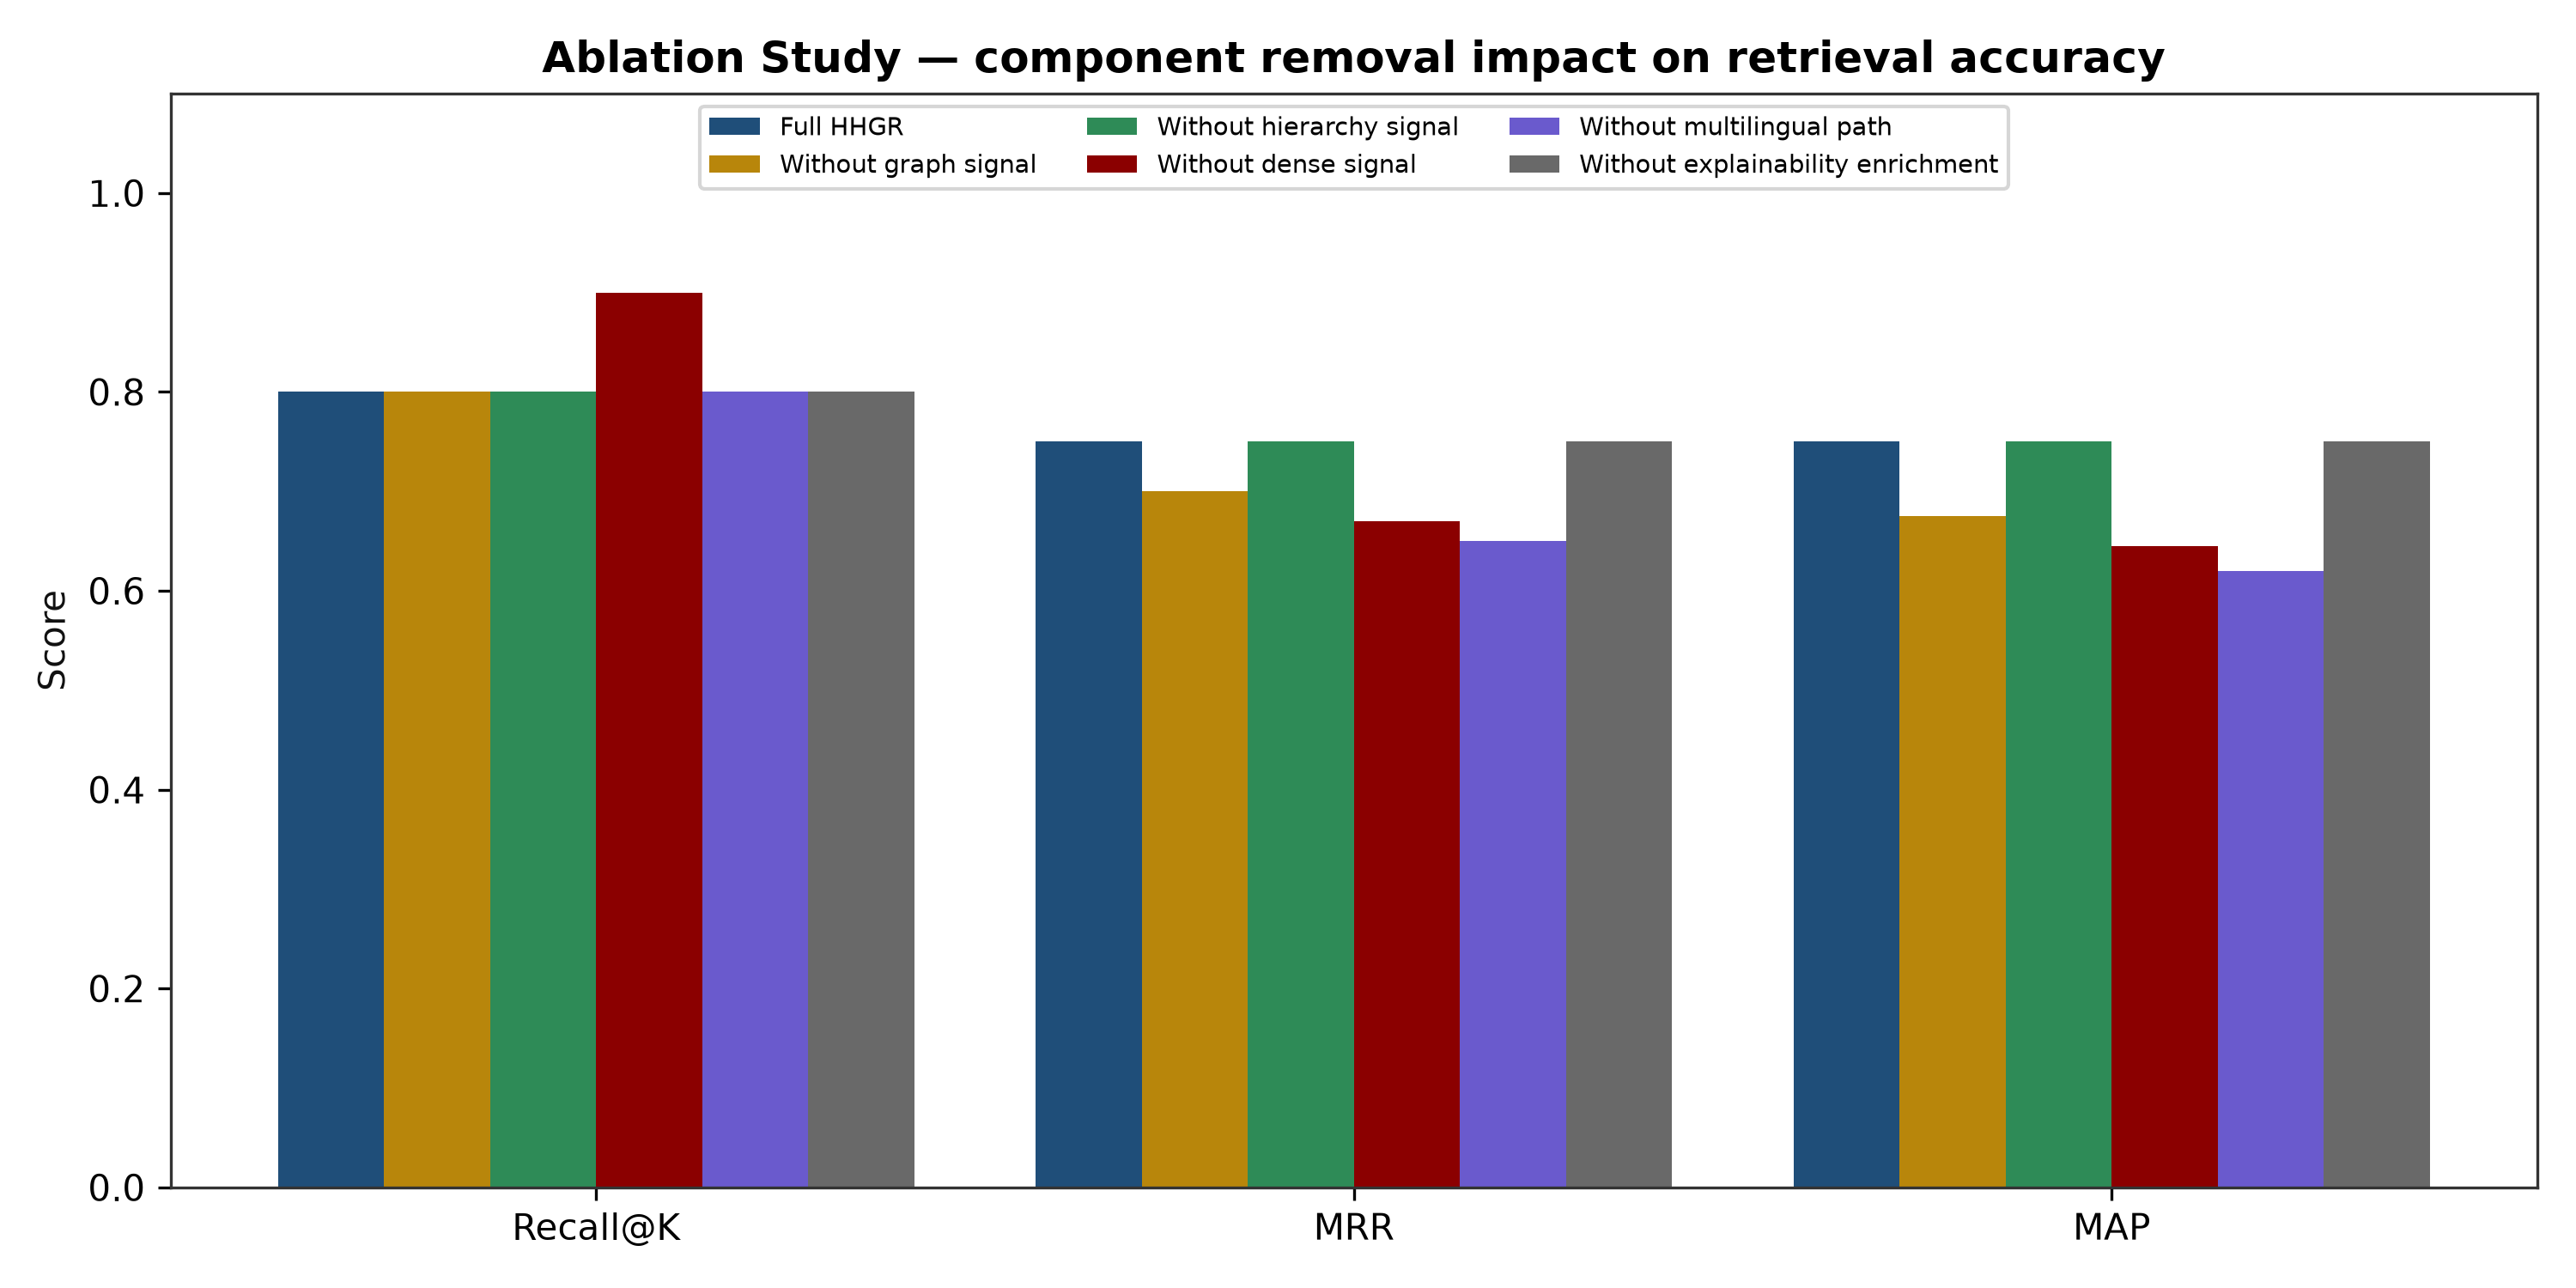
\includegraphics[width=0.9\columnwidth]{../evaluation/figures/ablation_chart.png}
\caption{Component-removal ablation on retrieval accuracy, generated by the
evaluation harness.}
\label{fig:ablation_chart}
\end{figure}

\subsection{Generation quality}

With the deterministic mock generator, both HHGR and Naive RAG achieve
faithfulness~1.0. Naive RAG reaches full citation-anchor context recall (1.0)
because its dense hits carry the exact gold section numbers, while HHGR covers
a broader, structurally enriched evidence set (0.75); answer relevancy and
correctness are comparable (0.78/0.44 vs.\ 0.82/0.46), reflecting the fact that
the mock answer is template-based. Real LLM deployments are expected to amplify
the provenance advantage.

\section{Future Work}

\begin{itemize}
  \item \textbf{Scaling the corpus}: extend evaluation to full statutes (BNS,
        BNSS, BSA), judgments, and the modern renumbering mappings between
        repealed IPC/CPC/Evidence Act provisions and their successors.
  \item \textbf{Real multilingual embeddings}: replace the deterministic
        provider with bge-m3 or LaBSE and evaluate cross-lingual transfer
        quantitatively, including Indic-language tokenization for coverage
        metrics.
  \item \textbf{Gold-answer generation}: replace the mock LLM with open or
        commercial models and run native RAGAS evaluation end-to-end.
  \item \textbf{Temporal validity}: model amendment and repeal edges as
        dated relations so counter-authority detection becomes provenance-based
        rather than marker-based.
  \item \textbf{Learned fusion}: replace fixed signal weights with a
        learn-to-rank model over the HHGR signal features.
  \item \textbf{Human evaluation}: collect lawyer assessments of citation
        usefulness, hierarchy correctness, and overall answer verifiability.
\end{itemize}

\section{Reproducibility}

All artifacts are included: the evaluation dataset under
\texttt{data/eval/gold/}, the experiment configuration under
\texttt{data/eval/config/}, the metrics and harness under \texttt{eval/}, and
the one-command script \texttt{scripts/reproduce.sh}, which installs the locked
requirements and emits every report and figure under \texttt{evaluation/}.


\section*{Acknowledgment}
The authors thank the open-source ecosystem for the libraries that power
Explaintool, including Neo4j, Qdrant, FastAPI, and Hugging Face Transformers.

\bibliographystyle{IEEEtran}
\bibliography{references}

\end{document}
